% This file was created by matplotlib2tikz v0.6.18.
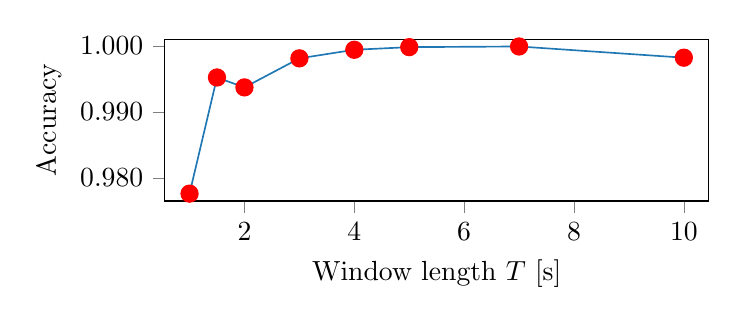
\begin{tikzpicture}

\definecolor{color0}{rgb}{0.12156862745098,0.466666666666667,0.705882352941177}

\begin{axis}[
height=0.3\textwidth,
width=0.7\textwidth,
tick align=outside,
tick pos=left,
x grid style={lightgray!92.026143790849673!black},
xlabel={Window length $T$ [s]},
xmin=0.55, xmax=10.45,
y grid style={lightgray!92.026143790849673!black},
ylabel={Accuracy},
ymin=0.976485, ymax=1.001015,
y tick label style={
        /pgf/number format/.cd,
            fixed,
            fixed zerofill,
            precision=3,
        /tikz/.cd
    },
    x tick label style={
        /pgf/number format/.cd,
            fixed,
            fixed zerofill,
            precision=0,
        /tikz/.cd
    }
]
\addplot [semithick, red, mark=*, mark size=3, mark options={solid}, only marks, forget plot]
table [row sep=\\]{%
1	0.9776 \\
1.5	0.9952 \\
2	0.9937 \\
3	0.9981 \\
4	0.9994 \\
5	0.9998 \\
7	0.9999 \\
10	0.9982 \\
};
\addplot [semithick, color0, forget plot]
table [row sep=\\]{%
1	0.9776 \\
1.5	0.9952 \\
2	0.9937 \\
3	0.9981 \\
4	0.9994 \\
5	0.9998 \\
7	0.9999 \\
10	0.9982 \\
};
%\path [draw=black, fill opacity=0] (axis cs:0,0.99038)
%--(axis cs:0,0.99962);

%\path [draw=black, fill opacity=0] (axis cs:1,0.99038)
%--(axis cs:1,0.99962);

%\path [draw=black, fill opacity=0] (axis cs:0.55,0)
%--(axis cs:10.45,0);

%\path [draw=black, fill opacity=0] (axis cs:0.55,1)
%--(axis cs:10.45,1);

\end{axis}

\end{tikzpicture}